\documentclass[norsk]{article}
\usepackage[utf8]{inputenc}
\usepackage[T1]{fontenc,url}
\urlstyle{sf}
\usepackage{babel,textcomp,csquotes,varioref,graphicx}
\usepackage{amsmath,pstricks,subfigure,fixltx2e,caption,epsfig,tikz,bookman}
\usepackage[backend=biber,style=numeric-comp]{biblatex}
\def\SB#1{\textsubscript{#1}}
\title{Hvordan kan man visualisere en overflate ved hjelp av Delaunay triangulering}
\author{Sølve Rene Johnsen}
\addbibresource{library.bib}
\begin{document}
\maketitle{}
\section*{Introduksjon}
Et kart, et ansikt, alle geometriske flater som vi ser dem, blir i dag
representert på datamaskinene. Man tenker kanskje ikke
over det, men når man tegner grafikk så er det oftest ingen forskjell
på en okse, et ansikt eller et kart når det kommer til metoden for hvordan man
illustrerer 3d flater. For mange lesere så har dere
allerede hatt erfaringer med enten å lete opp et kart via google maps
eller andre kartmodeller. Kanskje har dere spillt et skytespill og
inspisert ansiktet til personen du har valg og tenkt, ``hvordan
fungerer dette?''. Dette spørsmålet er essensen i oppgaven du skal
lese, hvor vi skal utrede, diskutere, og prøve å finne et svar på
dette.

\section{Begrepsdefinisjoner}
For å kunne forstå visse fagutrykk, blir dette avsnittet brukt til å 
definere de.
De forskjellige seksjonene er satt opp på en slik måte at de naturlig bygger
på tidligere definisjoner.

\subsection{Polygon}
Et polygon i geometri er en planlukket kurve sammensatt av et endelig
antall rette linjer. En trekant er derav det enkleste polygonet i et
plan.

\subsection{Trekant}
En trekant er et polygon med tre sidekanter og tre hjørner. Enhver
trekant har en entydig bestemt sirkel som går gjennom alle de tre
hjørnene i trekanten. Denne sirkelen kalles den omskrevne sirkelen til
trekanten eller også omsirkelen.  Avstanden fra den omskrevne
sirkelens sentrum s til de tre hjørnene p1, p2 og p3 er radiusen
til sirkelen. For hvert par av punktene p\SB{i} og p\SB{j} finnes det
en midtnormal l\SB{i},\SB{j} slik at ethvert punkt på
linjesegmentet, har samme avstand til p\SB{i} og til p\SB{j}. De tre
midtnormalene til kantene i trekanten skjærer hverandre i setrum til omsirkelen.
Se figur
\ref{trekant}

\begin{figure}
\centering
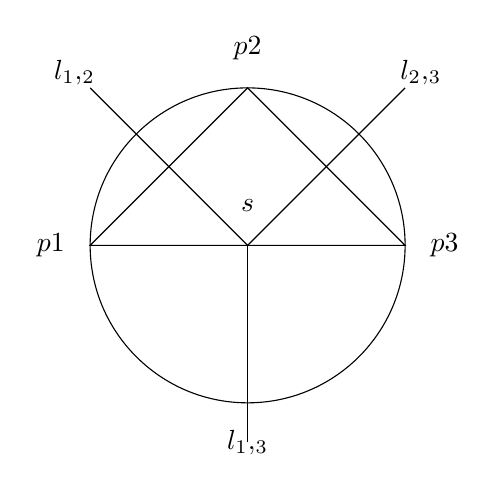
\begin{tikzpicture}
\draw (-2,0) -- (0,2) -- (2,0) -- cycle;
\node at (-2.5,0) {$p1$};
\node at (0,2.5) {$p2$};
\node at (2.5,0) {$p3$};
\node at (-2.2,2.2) {$l_1,_2$};
\node at (2.2,2.2) {$l_2,_3$};
\node at (0,-2.5) {$l_1,_3$};
\node at (0,0.5) {$s$};
\draw (0,0) circle (2cm);
\draw (0,-2.5) -- (0,0);
\draw (-2,2) -- (0,0);
\draw (2,2) -- (0,0);
\end{tikzpicture}
\caption{En trekant med 3 midtnormaler, og dens omskrevne sirkel}
\label{trekant}
\end{figure}

\subsection{Kollinearitet og kosirkularitet}
Hvis to eller flere punkter er på samme linje, sier vi at de
er kolineare. Om to eller flere punkter er på samme sirkel, sier
vi at de er kosirkulære.

\subsection{Triangulering}
Triangulering i geometri blir beskrevet som at en flate
representeres via en eller flere trekanter. Man kan tenke seg at man
starter med et antall spiker i et plan. Tar en strikk og strekker
den, slik at strikkens ytterpunkter er utenfor spikrenes ytterpunkter, for så
å slippe den. Strikken danner da et polygon, også kalt den konvekse
innhyllingen. Antall punkter langs det ytre polygonet er n, og antall inni er m.
Først så velger man vilkårlig av alle n punkter, ett punkt. Trekker så
kanter fra dette punktet til de n-3 motstående punkter, slik at man
får n + (n - 3) eller 2n - 3 kanter, og n-2 triangler. Så tar man for
hvert punkt m, og trekker linjer til punkter allerede triangulert,
slik at man får trekanter. Da får man 2n + 3*m - 3 kanter og n + 2*m -
2 antall triangler.

\subsection{Delaunay triangulering}
Boris Delone(1890 - 1980) var en russisk matematiker.  Delone fikk
sitt etternavn fra sin stamfar som i sin tid var en fransk offiser og
het De Launay. Boris Delone brukte heller Delaunay som etternavn i
offentlige publikasjoner og er kjent deretter.
\\\\
Delaunay triangulering handler om at for hver trekant i en triangulering 
skal man ikke ha flere punkter til denne trekantens omsirkel enn dem som
lager trekanten.
Som et resultat blir små vinkler større i trianguleringen.
Algoritmen som vi bruker omhandler å bygge opp Delaunay trianguleringen 
gradvis innover i grafen, man kan sammenligne det med 
bredde først søk, hvor man ser på trekanten man tegner sin omsirkel ikke har
noen andre trekanter i seg.
\subsection{Voronoi diagram}
Et Voronoi diagram omhandler å partisjonere områder mellom punktene slik at
ethvert punkt P\_i er omgitt av et polygon hvor alle punktene inne i
polygonet er nærmere P\_i enn alle andre punkter i P.
Voronoi og Delaunay er duale, ved duale menes at man kan gå fra en Delaunay
triangulering til Voronoi diagrammet og tilbake ved enkle algoritmer.
Skal man fra en Delaunay triangulering det duale Voronoi diagrammet tegner
tar man midtnormalen på alle trekantsidene hvor man som resultat får polygonene
beskrevet tidligere.
\\\\
\subsection{Høydekart}
Et høydekart er kort fortalt en måte å få en følelse av høyde i et
plan, dvs at hvert punkt har en z-verdi. Man kan oppnå dette med
skyggelegging i spill og fargekoter på kart.

\subsection{Flatemodell}
En flatemodell er en 3d representasjon av en flate. 
Man bruker det typisk til å illustrere terreng på jorda via kart, eller
gemetriske gjenstander på en skjerm via spill. Rutenett og triangulering 
er de mest hyppigst brukte metodene.

\subsection{Rutenett}
Rutenett eller grid, i kart sammenheng er bygget opp av bredde- og
lengdegrader som definerer koordinatssystemet og hvor det i hvert 
skjæringspunkt mellom bredde- og lengdegrad i grid er angitt en høyde(z-verdi)
ofte estimat fra omliggende målinger.

\subsection{Kartprojeksjon}
Siden jordkloden er ``rund'' har det gjennom historien vært vanskelig
å lage ett godt verdenskart. Man kan legge mange ulike og motstridende
krav til hva denne godheten er. I denne oppgaven skal vi se på
følgende krav: Hvis man på et kart trekker en linje fra A til B og
så får man en kompasskurs, så kan følge denne f.eks når man seiler. 

\subsection{Mercator}
Geraruds Mercator kjent i dag for Mercator projeksjon som er en
sylindrisk kartprojeksjon presentert i 1569.  Denne ble til den mest
brukte kartmodellen fordi den oppnår kravene nevnt i Kartprojeksjon
som omhandler å kunne holde en rettlinjet kurs, feks med et skip.
Hvis man tenker seg at man putter en kule K i en sylinder S hvor K sin
omkrets treffer S sine vegger altså tangenserer. Deretter tenker man
kulen K sitt midtpunkt P som projeserer ut for alle landmasser L i K
ut på planet i S. Om man da bretter ut sylinderet får man da, ett godt
nok ,representativ kart over K.

\section{Formålet med oppgaven}
Formålet med oppgaven er, gitt en punktliste med formen x,y og z og videre lage
gode visualiseringer av de. Det skal lages modeller av overflater, ikke volumer.
Jeg har vært så heldig at jeg har fått gitt et program som gir meg delaunay
trianguleringen gitt en punktliste. 
Hvis punktlistene representerer et kart, skal det trekkes koter og fargelegge
i forhold til høyde.
Om det er figurer som mennesker eller andre former, skal det skygge- og 
fargelegges i forhold til høyde. 
Tanken er at man skal kunne dreie på flaten, slik at det tegnes
opp på nytt. Det er viktig at man effektiviserer ved å unlate å tegne opp
ikke synlige detaljer, også kalt klipping som underkategoriseres
 ``generalisering'', under seksjonen ``Budskapet i en fremvisning''.

\subsection{Visualisering}
Visualisering vil si å synliggjøre. Mennesker egner seg dårlig til å trkke
nyttig informasjon via tall, men så fort det blir omgjort til bilder i form av
kurver i 2d flater eller volumer i 3d, kan vi bruke synssansen til å dedusere
informasjonen som leder til bedre forståelse. Derfor er det viktig å kunne
rotere, zoome ut og inn i sanntid slik at viktige detaljer på en gjenstand
kommer med, som f.eks hanken på en kopp eller bruen over en elv. Gjenstander som
ville blitt oversett i gitte vinkler.

\subsection{Fra 3d til 2d}
Man får matriser gitt, hvor man har et bilde man vil vise som skal representere
informasjonen. Det første man gjør er å klippe bildet slik at bare informasjon
som kan visualiseres, vises. Deretter vil man projisere den 3dimensjonale scenen
ned til en flate via teknikker tidligere diskutert. Så må man gjøre det om til
piksler på skjermen, eller rasterisering.

\subsection{Begrensninger med rasterisering}
Når man har en skrå linje via en gitt matrise så vil denne skrå linjen bli
representert med en mer trappeformet linje med pikselrepresentasjon. Denne
effekten kalles aliasing. Grafikkort i dag har innebygd støtte for å redusere
problemet, teknikken heter antialiasing. Antialiasing går ut på å glatte ut
skarpe fargeoverganger ved å blende inn bakgrunnsfargen i kantene til det
geometriske objektet.

\subsection{Vektorisering}
Gitt en oppløsning x så rasteriserer man, hvis man da zoomer inn eller ut så 
blir oppløsningen x justert opp eller ned og man vil da rasterisere på nytt.
Forskjellen på direkte rasterisering og vektorisering er som forskjellen på
statisk og dynamisk. Hvis man zoomer inn på et jpeg bilde vil man se pikslene
fordi bildet ikke blir tegnet opp på nytt. Zoomer man inn på et png eller pdf
bilde blir bildet tegnet opp i forhold til oppløsningen. Vi skal bruke
vektorisering.

\section{Budskapet i en fremvisning}
Når man er ute etter å selge et bord via annonse og man har tilgang til et bilde
som viser bordet. Er det viktig at fokuset i bildet er bordet og ikke hva som
ligger på bordet eller hva som er i bakgrunnen til bordet. Dette kan også sees på som å formidle budskapet i et bilde på en mer effektiv måte. Det finnes flereteknikker for å gjøre dette. For å vite om disse teknikkene må vi forstå
generalisering. Beskrevet i neste avsnitt.

\subsection{Generalisering}
Tenk deg at du går inn i en skog og setter deg på en stein. Du ser deg omkring
og bruker alle sanser, du fokuserer litt på å høre fuglene som kvitrer, og så
litt på å se litt på busker og trær. Det neste som skjer er kanskje at du
lukter granen som står rett ved siden av deg. Alle disse tankene skjer
sekvensielt og er essensen i hvordan menneske hjernen fungerer, det som egentlig
skjer er at vi generaliserer omgivelsene på bakgrunn av hva vi fokuserer på.
Generalisering betyr å få ned detaljer i et gitt innhold slik at budskapet
eller kriteriene til innholdet blir bevart og/eller fremhevet. Dette er en
teknikk som er essensen i menneskets rasjonalisering og logikk. En logikk 
også brukt i kartsammenheng kalt kartgeneralisering som beskrevet i neste avsnitt.

\subsection{Kartgeneralisering}
Kartgeneralisering handler om å få frem detaljer man vil fremvise på en
måte slik at man fortsatt bevarer virkeligheten på en gjenkjennelig måte.
Noen metoder for å gjøre dette blir beskrevet under.

\subsubsection{Utvalg}
Utvalg handler om å redusere data ved å velge ut unødvendige detaljer i forhold
til agenda.

\subsubsection{Forenkling}
Utvalg inngår også i forenkling, hvor man velger ut unødvendigheter, men 
forenkling omhandler om å gjøre data mindre detaljert og mer synlig.

\subsubsection{Glatting}
Glatting handler om å glatte ut linjer slik at det blir mer forståelig, på samme
tid som man bevarer virkeligheten godt nok.

\section{Kartfremvisning}
For å forstå et kart må det lages på en intuitiv måte slik at brukeren
raskt kan dedusere informasjon som fjell, daler, vann, stier, byggninger og mer.
De hyppigste teknikkene brukt for å illustrere høyde i et terreng er ved bruk
av farger. Hvis man tenker seg en delaunaytriangulering av et geografisk
området så vil ikke tall og rette linjer si oss så mye. Om vi fargelegger 
alle områder mellom 0 - 50 m.o.h med lysegrønn, alt mellom 51 - 150
m.o.h med en mer mørk grønn så vil vi allerede raskt deduserer hvor vi har
bakker og daler. Å fargelegge trianguleringen gitt, er noe som skal gjøres i 
denne oppgaven.

\subsection{Fire farge teoremet}
Jeg tenkte det kunne være lurt å følge fire farge teoremet, som går ut på at i et plan så kan man fargelegge alle områder slik at ingen samme farge grenser til hverandre, dette fordi det er veldig hyppig brukt og lett å gjenkjenne.

\section{Figurfremvisning}
Som beskrevet i over i seksjonen ``Kartfremvisning'' så skal man bruke samme
teknikker, men for å kunne illustrere dybde i et menneskeansikt, vil man
vise nesen som en lysere hudfarge, og innhylninger som kinn vil skyggelegges
og en litt mørkere nyanse av samme hudfarge vil brukes.

\section{Løgnfaktor}
Løgnfaktor handler om forholdet mellom det å illustrert i grafikk i forhold til
data. Så hvis G står for mengden av elementer i grafikk og D for mengden av
elementer i data, slik at |G| = |D|. Da er løgnfaktoren lik forholdet mellom
2 vilkårlig valgte elementer i G delt på 2 elemente med samme posisjon i D
Hvis verdien valideres til 1 så er mengdene like og grafikken representerer 
dataen troverdig. Blir verdien mindre enn 1 så underdriver grafikken dataen,
mer enn 1 så overdriver grafikken dataen.
I denne oppgaven skal man alltid ha en løgnfaktor tilnærmet lik 1. Tilnærmet
fordi hvis man glatter linjer så vil noen verdier ikke være like.  

\section{Ideer til masteroppgave}
Jeg har tenkt på å lage et kart program som først tar inn en ferdig laget 
delaunay triangulering gitt en punktliste. Slik at man trekker koter ved
visse høyder på kartet og fargelegger disse. Hvordan det skal fargelegges
kan avgjøres siden. Videre ideer kan leses på i de neste avsnittene.

\subsection{Roterbart landskap med filter}
At man skal kunne dreie på landskapet slik at man får flere perspektiv og
forståelse av hva man ser på, slik at tegner opp landskapet for hver 
dreining.
At man skal kunne legge på flere filter i forhold til annen informasjon gitt,
hvor et filter kan være økonomi, slik at landskapet blir forstørret eller 
forminsket basert på inntekt per innbygger.
Et annet filter man kanskje kunne lagt på kunne vært innbyggertall, hvor
landskapet ville blitt større eller mindre basert på innbyggertall.
Man kunne også hatt et filter hvor man kunne basert på etnisk bakgrunn
gjort landskapet større eller mindre.
En annen ide kunne vært basert på utslipp og forurensning. Det finnes flere
filter ideer som kan utforskes, men det kunne vært en god fremvisning av
data for å se om det finnes korelasjoner mellom dem.

\subsection{Roterbart landskap med Byggefilter}
En ide kunne vært at jeg hadde lagt opp slik at man kunne satt inn
et filter med arealet a og en maks høydedifferanse h. 
Slik at landskapet viser alle områder som oppfølger kriteriene a og h. 
Dette kunne vært et interresant forretnings konsept fordi da kan man raskt se hvor man kan bygge.

\subsection{Roterbart landskap med stridsvognfilter}
At man skal vise alle posisjoner på et kart med et gitt antall kriterier som
for eksempel dekke av fjell, mindre synlig fra gitte posisjoner, taktiske
muligheter for å kunne både kjøre fremover og flykte i forhold til en annen 
posisjon, f.eks andre stridsvogner.
At ved en gitt posisjon så skal det vises hvor svakhetene er i forhold til å
ikke bli sett, å kunne se i alle retninger, å bli sett uten å kunne se i form
av forskjellige farger. Ruter for hvordan man bør kjøre for å ikke bli sett
av motstandere ved en gitt posisjon. Hvor man kan skyte fra uten å bli sett.
Det kunne kanskje bli brukt for flyangrep for å vise gode muligheter for
hvor stridsvogner kan befinne seg, slik at en datamaskin skanner disse 
områdene først når man flyr over. 

\section{Forskjellige java biblotek som kan brukes}
Jeg har gjort undersøkelser på forskjellige gratis biblotek som finnes for
å tegne opp og fargelegge. Og det skal utredes litt mer om mulighetene bak
de forskjellige biblotekene i de kommende avsnittene.

\subsection{Java.awt.Graphics, enkel grafikk manipulasjon}
Dette er et enkelt biblotek hvor man kan gjøre tegne operasjoner for så å
illustrere dette. Man må definere farger, hvilket koordinat man vil tegne
på og hva man vil tegne. Med denne klassen burde tegningen være grei nok
til mitt formål.

\subsubsection{Tegne en linje}
java.awt.Graphics.drawLine(int x1, int y1, int x2, int y2) slik at en rett
linje blir tegnet mellom <x1,y1> som er start posisjon og <x2,y2> som er 
slutt posisjonen.

\subsubsection{Tegne geometriske former}
drawLine,drawArc,drawRect,drawOval og -java.awt.Graphics.drawPolygon
for å tegne predefinerte geometriske former.

\subsubsection{Sette inn bilder}
java.awt.Graphics.drawImage(Image img, int x, int y, Imageobserver observer)
slik at bildet ``img'' settes til posisjonen gitt <x,y>, ``observer'' settes
oftest til ``null'' siden observer ikke skal brukes.

\subsubsection{Tegne tekst}
java.awt.Graphics.drawString(string tekst, int x, int y) for å tegne
``tekst'' inn i posisjonen <x,y>.

\subsection{javax.swing.JFrame, enkel måte å lage vindu på}
Ved å bruke JFrame får man et enkelt vindu som man kan bruke til å 
legge vårt grafikk bilde inn i. Man må først sette opp vinduet til hva det
skal hete, hvilken oppløsning det skal vises i.
Verdt å legge merke til er at JFrame ikke er ``thread-safe''


\printbibliography
\end{document}
